\begin{mydef}
	La médiatrice d'un segment est la droite \kw{perpendiculaire à ce segment} et qui \kw{passe par son milieu}.
\end{mydef}


\begin{myex}
	La droite $(d)$ est la médiatrice du segment $[AB]$.
	
	\begin{center}
		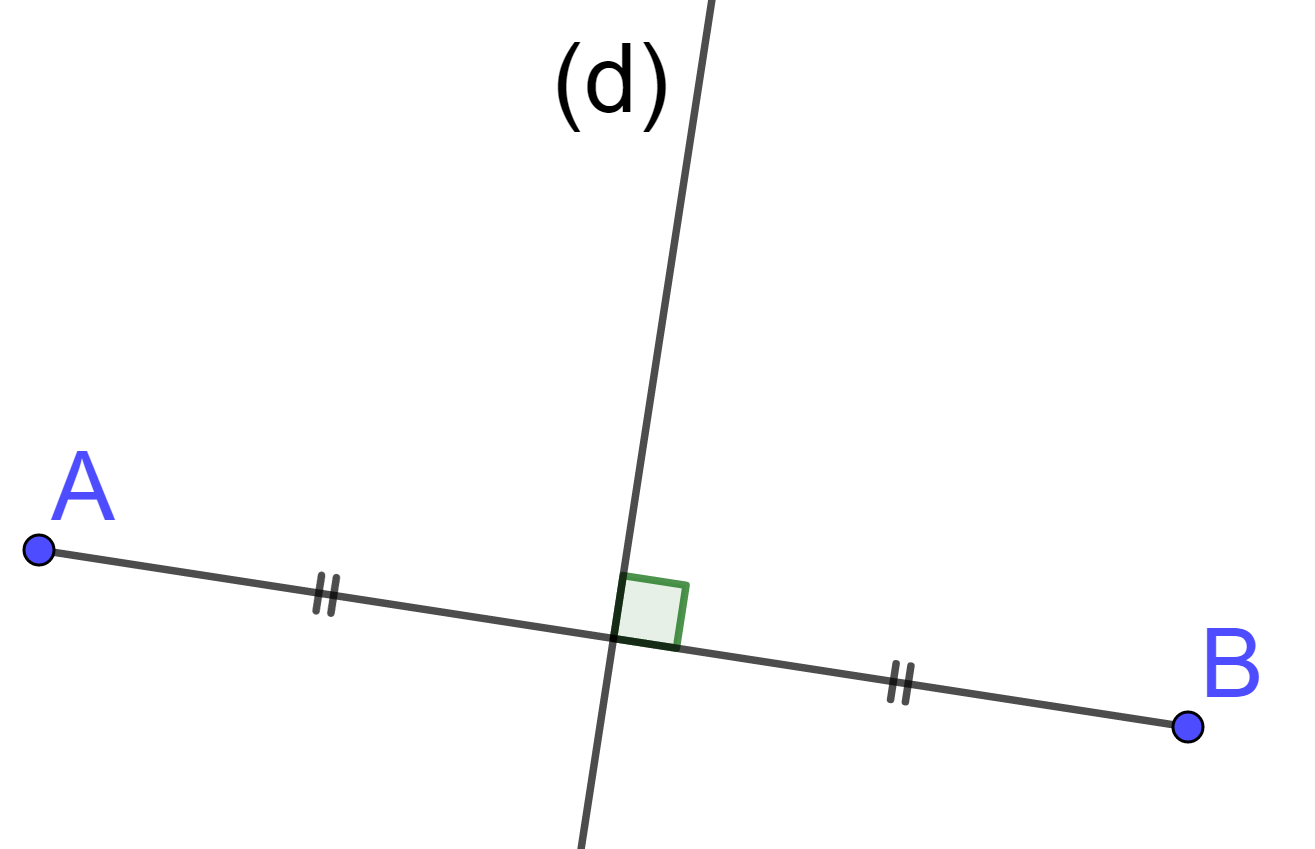
\includegraphics[scale=0.15]{med1}
	\end{center}
\end{myex}

\begin{myprops}
	\begin{itemize}
		\item \textbf{Si} un point appartient à la médiatrice d'un segment, \textbf{alors} ce point est à la même distance des extrémités de ce segment.
		\item \textbf{Si} un point est à la même distance des extrémités d'un segment, \textbf{alors} il appartient à la médiatrice de ce segment.
	\end{itemize}
\end{myprops}


\begin{myexs}
	\begin{multicols}{2}
		
		\begin{enumerate}
			
			
			\item  Le point $D$ appartient à la médiatrice $(d)$ du segment $[AB]$, donc $AD=BD$.
			
			\vspace*{0.5cm}
			\begin{center}
				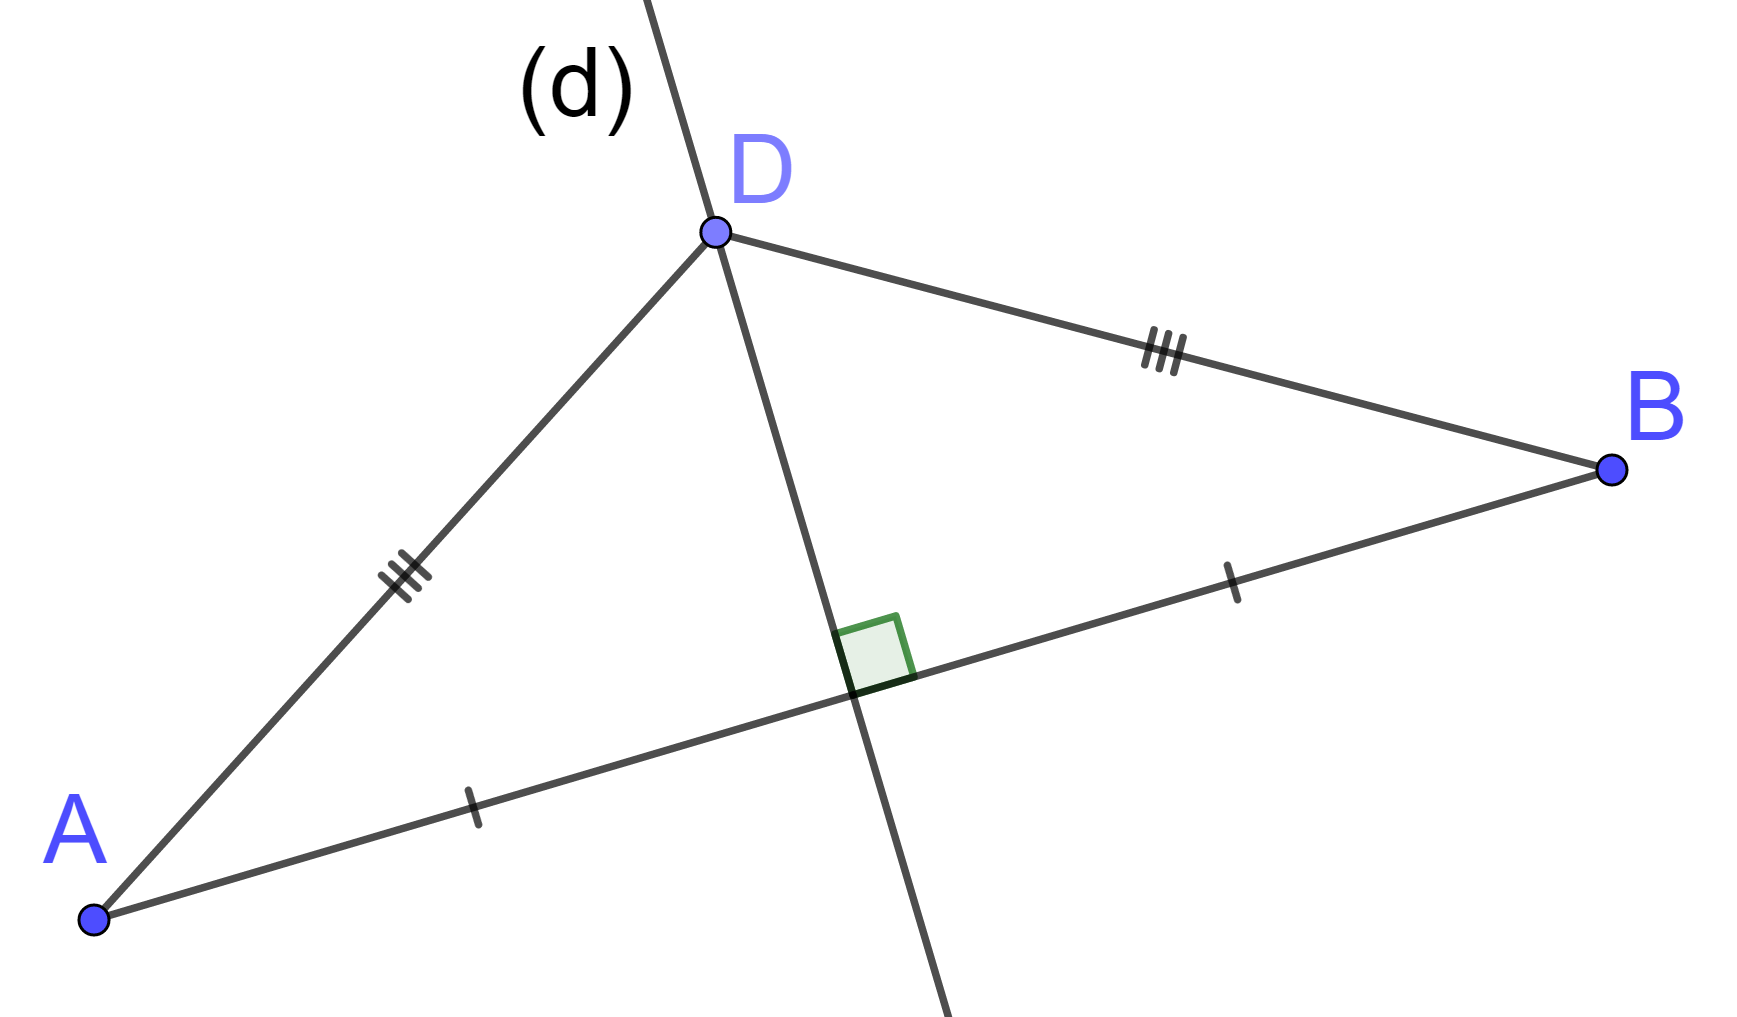
\includegraphics[scale=0.15]{med2}
			\end{center}
			
			
			\item On a $EG=GF$, $EH=HF$ et $EI=IF$, donc les points $G$, $H$ et $I$ appartiennent tous à la médiatrice du segment $[EF]$.
			
			\begin{center}
				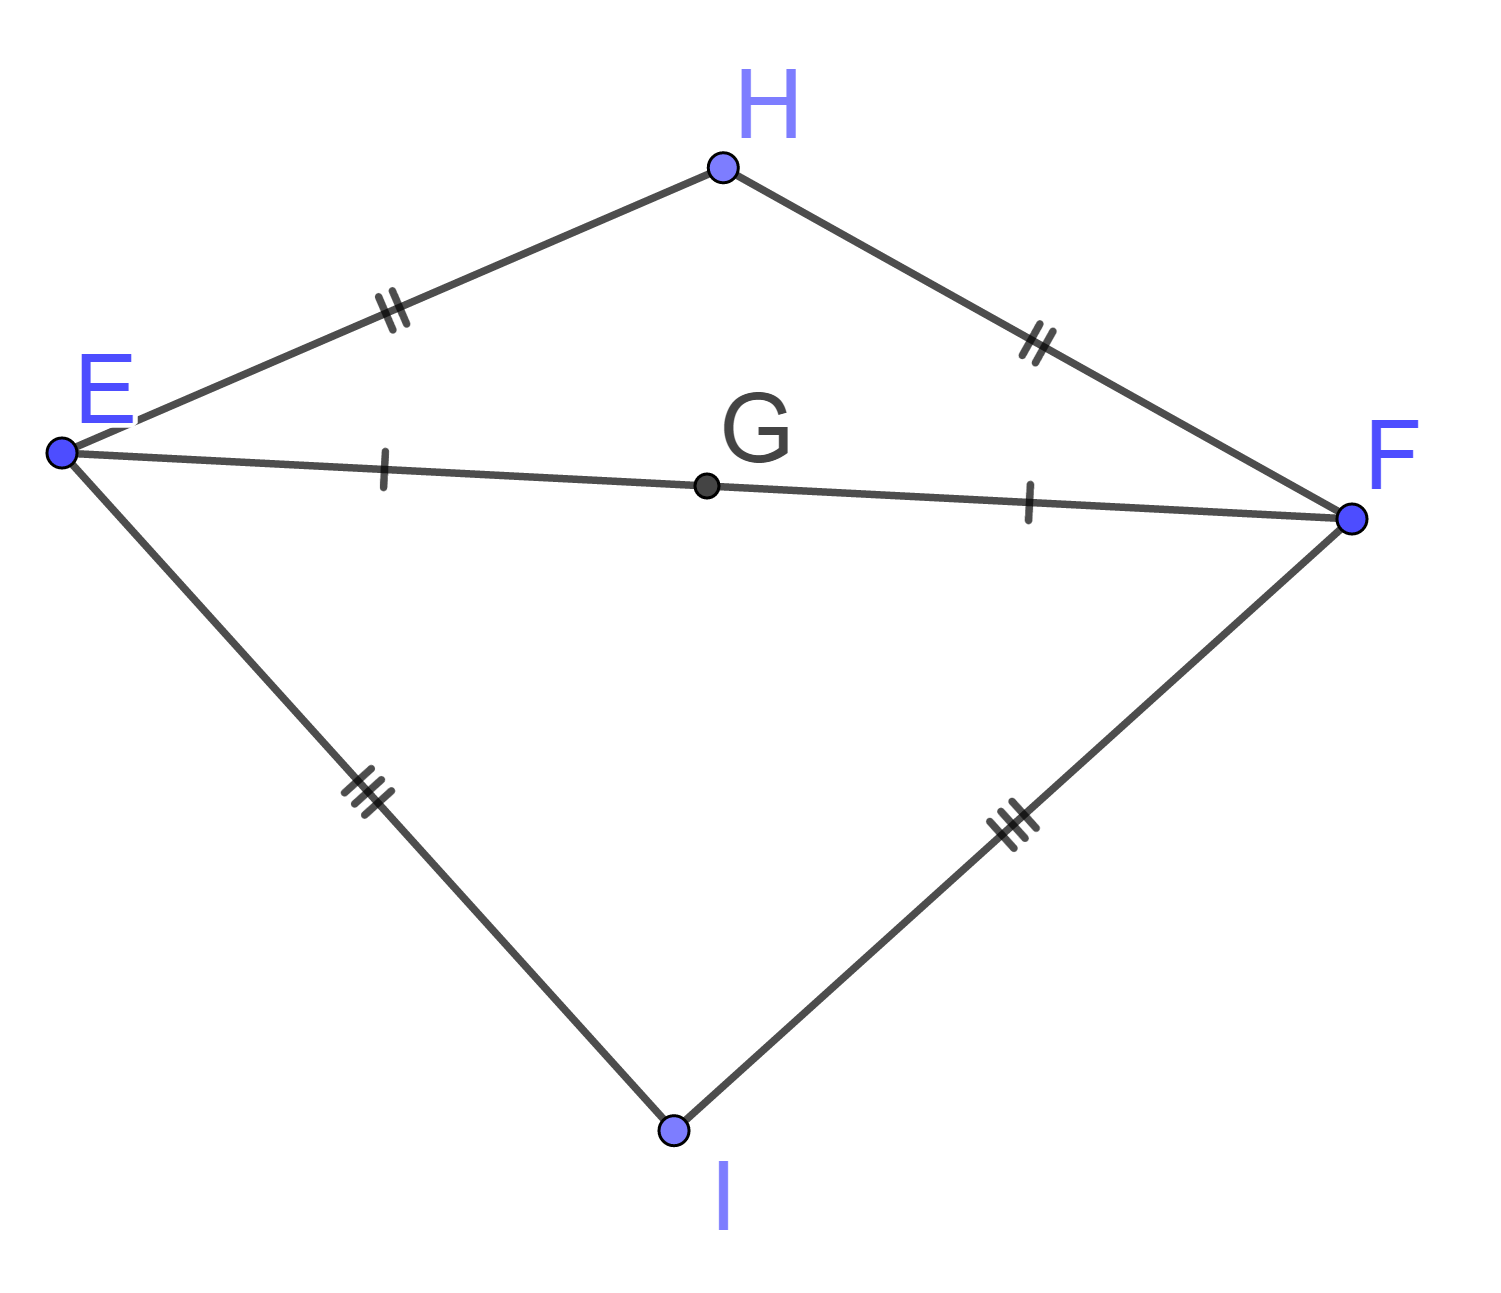
\includegraphics[scale=0.13]{med3}
			\end{center}
			
		\end{enumerate}
	\end{multicols}
	
	
	
\end{myexs}

\begin{mymeth}
	Pour tracer la médiatrice d'un segment $[AB]$ au compas et à la règle non graduée :
	
	\begin{enumerate}
		\item choisir un écartement plus grand que la moitié du segment;
		\item placer la pointe du compas en $A$ et tracer un arc de cercle;\label{step1}
		\item en gardent le même écartement, placer la pointe du compas en $B$;
		\item tracer un arc de cercle qui coupe le premier;
		\item placer le point $I$ à l'intersection;\label{step2}
		\item refaire les étapes \ref{step1} à \ref{step2} avec un autre écartement en nommant le point $J$;
		\item tracer la droite $(IJ)$ médiatrice du segment $[AB]$.
		
	\end{enumerate}
\end{mymeth}